\chapter{系统设计}
\thispagestyle{fancy}
本章主要介绍系统的功能设计,界面设计和架构设计。

\section{功能设计}
用户可以在主页上浏览一个按讨论数排序的话题列表。我们将一个话题的讨论数定义为微博中出现该话题的微博数。我们为每个话题定义了正则表达式,当一条微博中的字符串匹配了话题的正则表达式,就认为它出现了该话题,一条微博中多次匹配只计一次。

用户可以浏览一个话题的下列信息:
\begin{itemize}
\item 话题的简介;
\item 出现该话题的热门微博 (指评论数和转发量总和较多的微博);
\item 该话题讨论数随时间变化(以天为单位)的折线图;
\item 该话题讨论数在各省分布的地图;
\item 该话题中出现的情绪词云图;
\item 该话题的情绪特征柱状图;
\end{itemize}

情绪词是我们参考心理学家的相关研究(Ekman 六类基本情绪\cite{ekman71}, GPOMS 心境量表\cite{gpoms11}及中文情绪形容词检测表\cite{zj05})定义的词汇,如开心,失意,生气等。我们统计某话题下情绪词出现的次数,包括一条微博中出现的所有情绪词。
我们将这些情绪词分为快乐,悲伤,愤怒,恐惧,惊奇,厌恶和其他这七类情绪特征,并展示情绪特征的出现次数。

\section{界面设计}
用户通过 Web 界面访问我们的系统。界面总体上分成左右两栏:左侧为导航栏,右侧为内容栏。

在首页上,导航栏显示的是热门话题和话题分类选项及搜索框。内容栏显示的是根据话题讨论数排序的话题列表。列表中的一项包括话题名称和话题的讨论数。内容栏右下角提供向前向后翻页按钮。如图 3-1 所示。

\begin{figure}[!h]
\centering
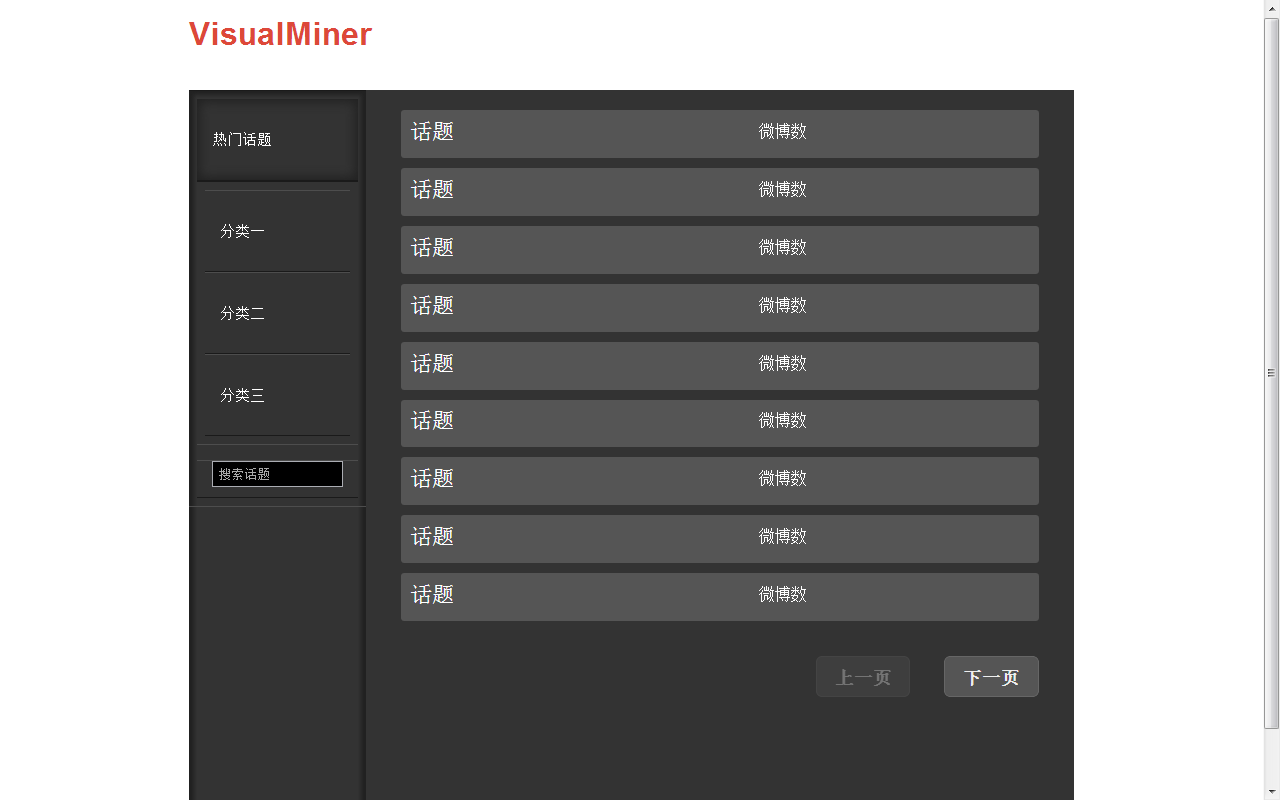
\includegraphics[width=\textwidth, height=0.4\textheight]{web_main}
图 3-1 主页
\caption{Home Page}
\end{figure}

在用户点击某个话题后,界面跳转到该话题的页面。此时内容栏分为上下两部分,上面固定显示话题的介绍,下面是可视化栏。导航栏提供热门话题,事件概况,情绪特征,地域特征,变化趋势 5 个选项。点击热门话题,回到话题列表页面。点击其余选项,可视化栏显示相应页面。默认展示的是事件概况页面。

事件概况页面上显示出现该话题的热门微博。如图 3-2 所示。

\begin{figure}[t]
\centering
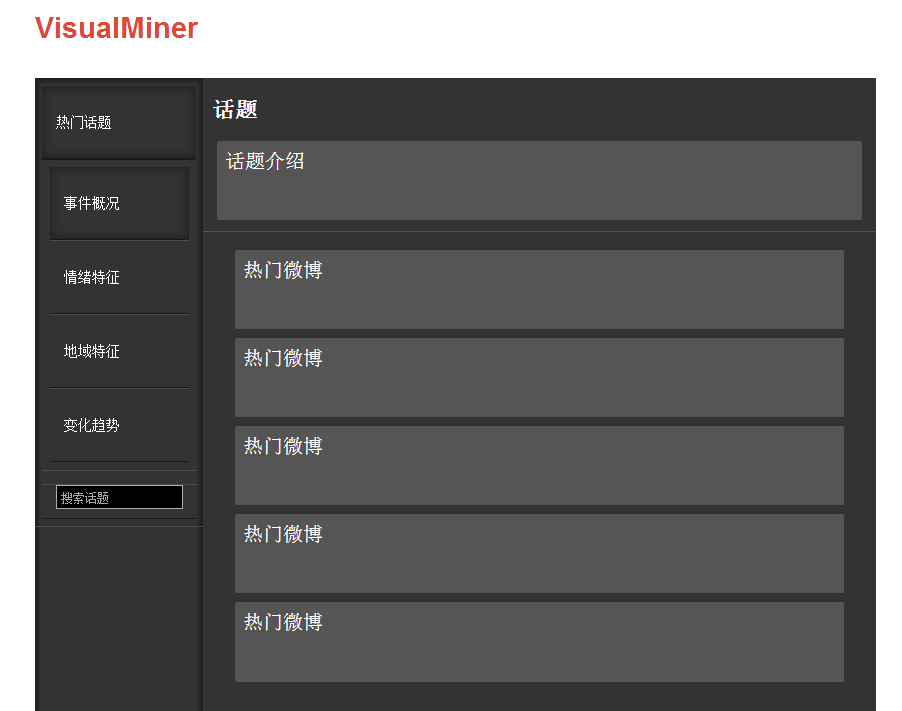
\includegraphics[width=\textwidth, height=0.37\textheight]{web_topic}
图 3-2 事件概况
\caption{overview}
\end{figure}

在导航栏上点击情绪特征,可视化栏进入情绪特征页面。该页面左侧为情绪特征柱状图,右侧为情绪词云图。如图 3-3 所示。
\begin{figure}[!h]
\centering
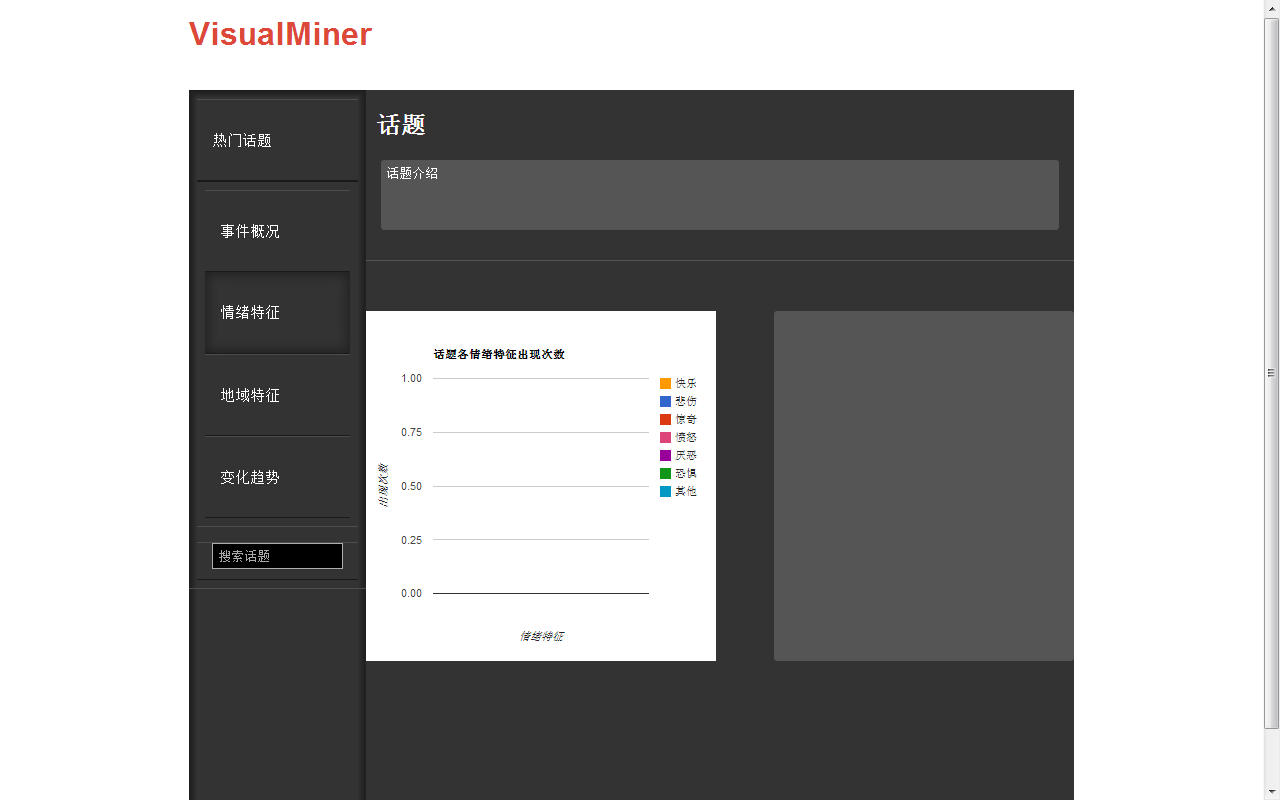
\includegraphics[width=\textwidth, height=0.37\textheight]{web_emotion}
图 3-3 情绪特征
\caption{emotion}
\end{figure}

在导航栏上点击地域特征,可视化栏进入地域特征页面。该页面显示按省划分的地图。一个区域填充色的深浅表示该区域出现该话题的微博数。当用户将鼠标移到一个区域上时,可以显示具体数值。如图 3-4 所示。
\begin{figure}[!h]
\centering
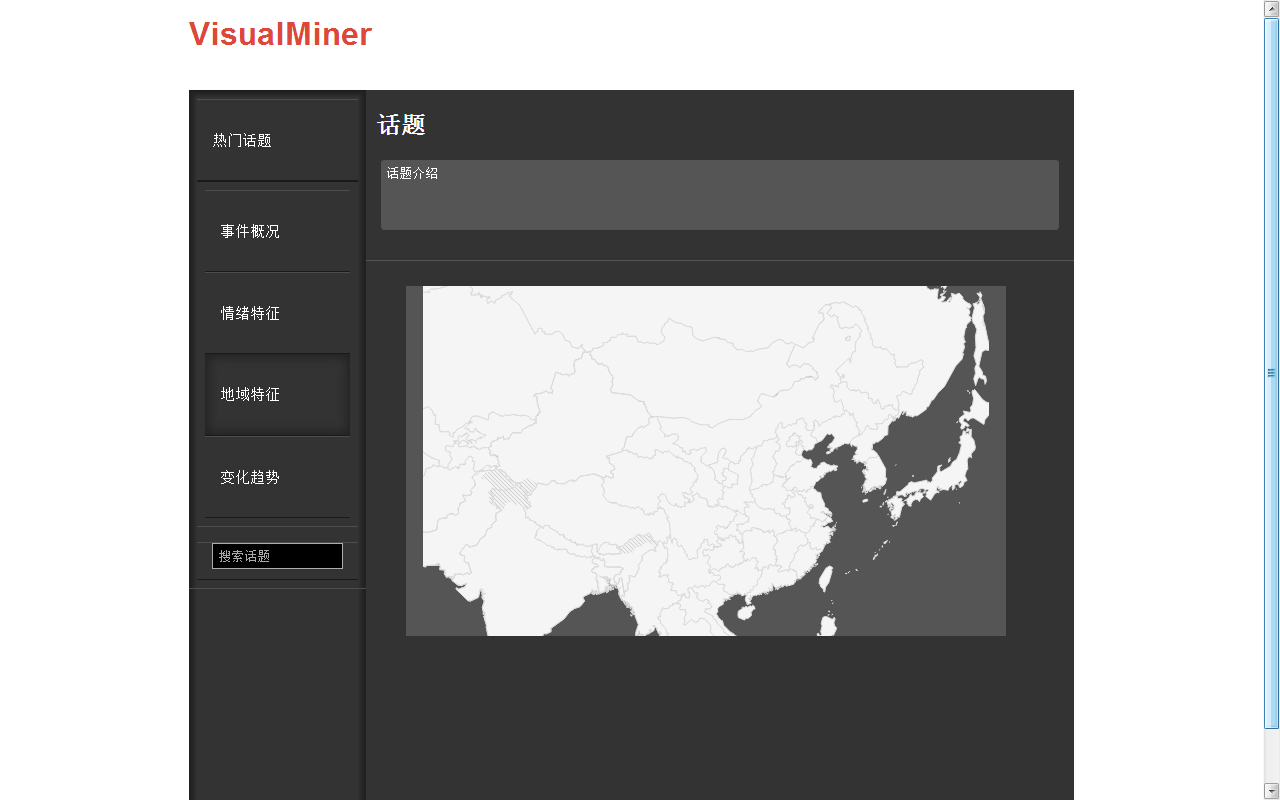
\includegraphics[width=\textwidth, height=0.37\textheight]{web_location}
图 3-4 地域特征
\caption{location}
\end{figure}


在导航栏上点击变化趋势,可视化栏进入变化趋势页面。该页面显示对话题的讨论数随时间变化的情况,用折线图表示,当用户将鼠标移到一个点上时可以显示具体数值。如图 3-5 所示。
\begin{figure}[!h]
\centering
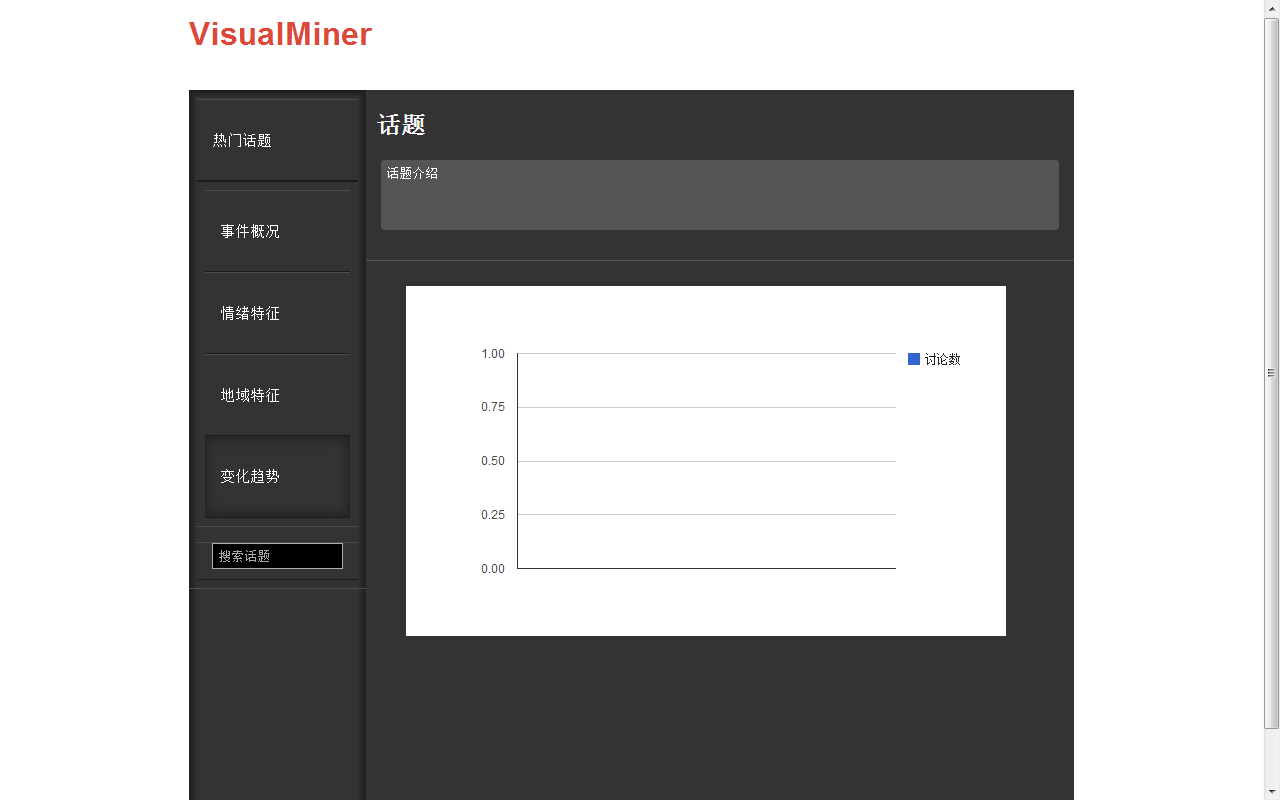
\includegraphics[width=\textwidth, height=0.37\textheight]{web_time}
图 3-5 变化趋势
\caption{trend}
\end{figure}

以上所有的界面都在一个 HTML 页面上,由 jQuery 实现动态页面跳转。

\section{架构设计}
系统架构如图 3-6 所示,总体上分成三个模块:数据获取模块,数据分析模块和数据呈现模块。

\begin{figure}[t]
\centering
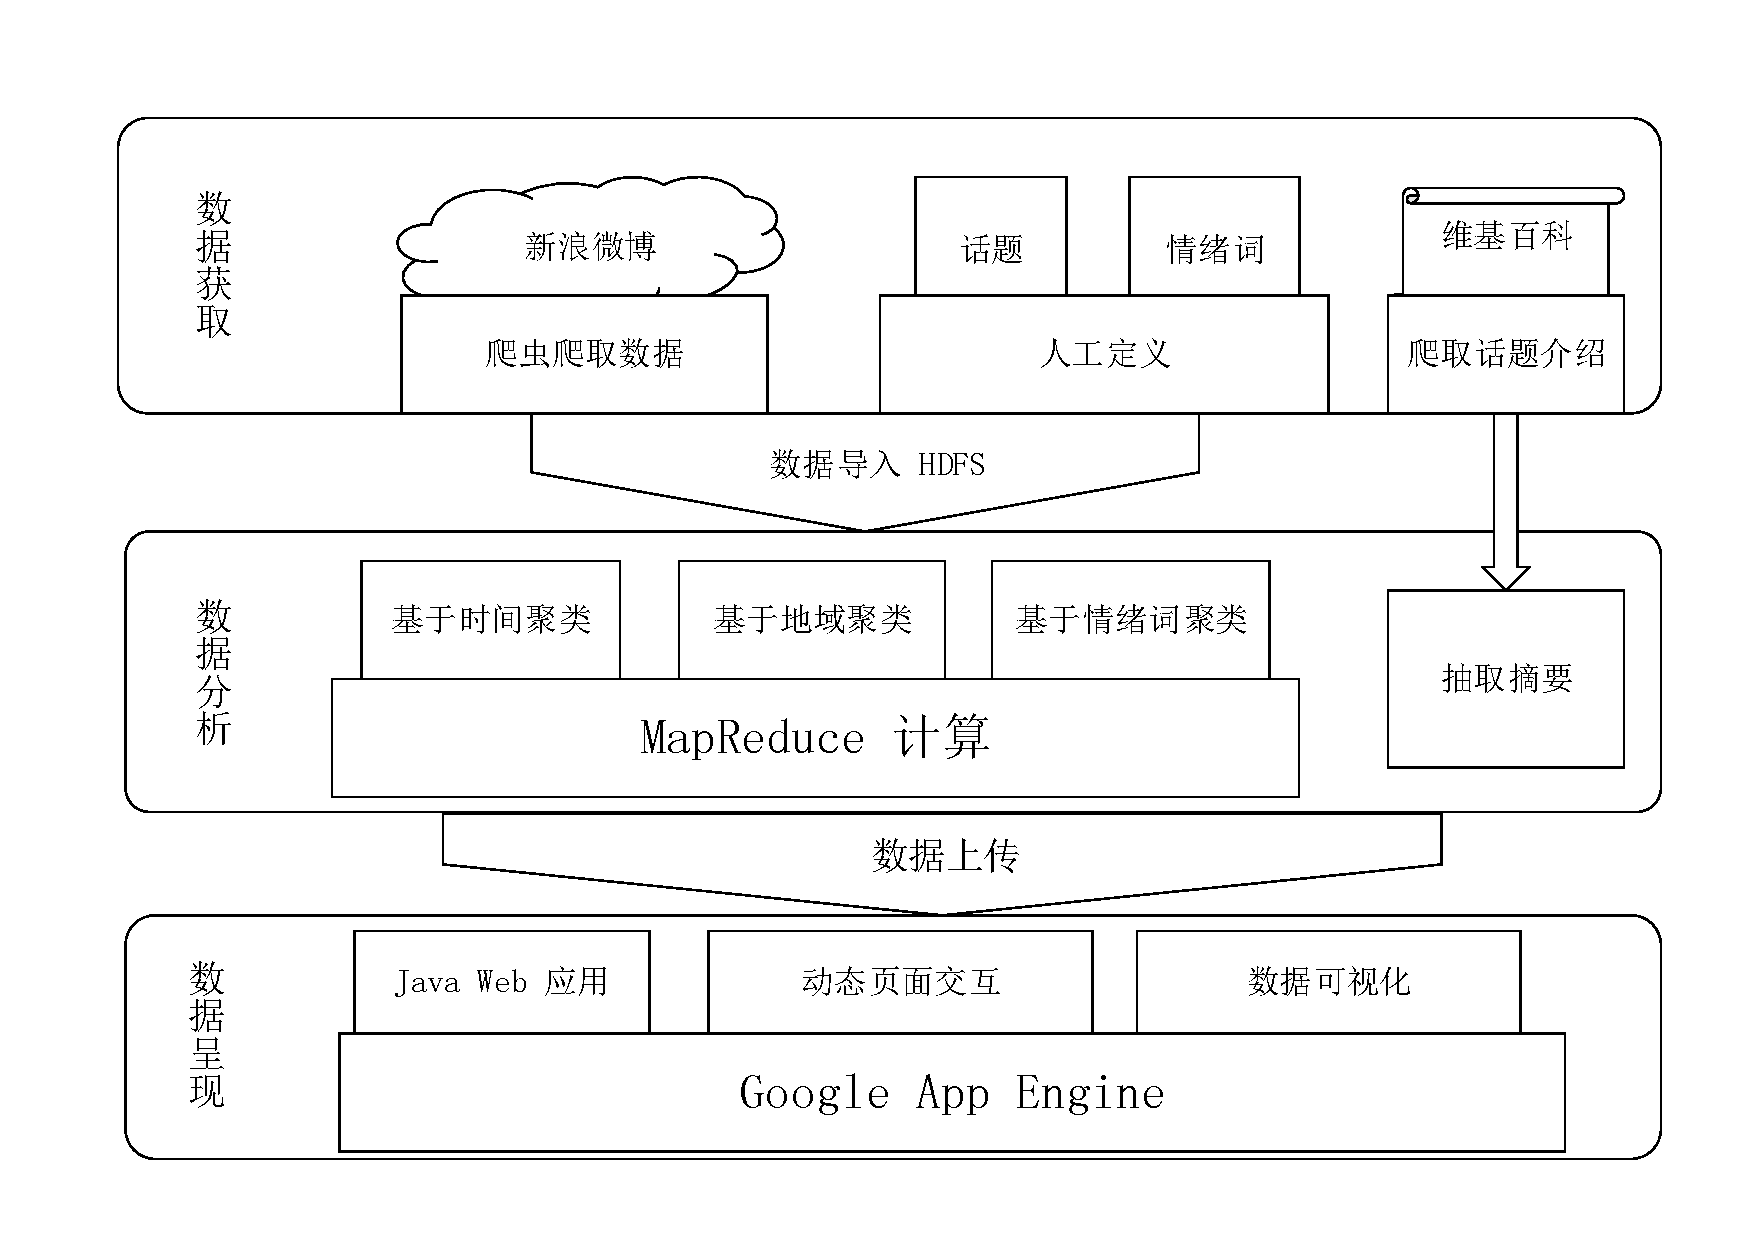
\includegraphics[width=\textwidth]{arch_min}
图 3-6 系统架构
\caption{system architecture}
\end{figure}


\subsection{数据获取模块}
数据获取模块分为三个部分:
\begin{itemize}
\item 第一部分,设计爬虫爬取新浪微博数据。
\item 第二部分,根据曾在新浪微博上引起广泛关注的话题定义话题列表,基于心理学家的相关研究定义情绪词和情绪特征。
\item 第三部分,通过 MediaWiki API 从维基百科爬取话题的介绍页面。
\end{itemize}
我们将前两部分数据导入 HDFS,用于下一阶段的 MapReduce 分析,第三部分的数据用于下一阶段抽取话题的简介。

\subsection{数据分析模块}
数据分析模块分为两个部分:
\begin{itemize}
\item 第一部分,我们应用 MapReduce 计算框架分析微博数据,在时间,地域,情绪等维度上对微博数据进行分组聚合。
\item 第二部分,我们从爬取的维基百科页面中抽取第一段话,用作话题的简介。
\end{itemize}
我们将两部分计算结果上传到 Google App Engine 的数据存储区。我们选用 High Replication 存储区存储数据,虽然其写入时的延时较高,但我们的系统在批量导入数据后只需要响应读操作,而它提供的高可靠性,保证不会因为机器崩溃导致用户无法访问,影响用户体验。我们的查询是基于键(话题)的,而不是基于关系的,所以我们没有选择传统的关系型数据库\cite{database}。

\subsection{数据呈现模块}
我们在 Google App Engine 上构建 Java Web 应用,利用 jQuery 实现动态用户界面和 Ajax,调用 JavaScript 库 (Google Chart Tools\cite{gct},Data-Driven Documents\cite{d3}等)可视化数据。





